\documentclass[12pt]{article}   % list options between brackets
\usepackage{graphicx}

% type user-defined commands here

\begin{document}

\title{CS288 Assignment 2: Phrase Translation}   % type title between braces
\author{Reynold Shi Xin}         % type author(s) between braces
\date{rxin@cs.berkeley.edu}    % type date between braces
\maketitle

%%%%%%%%%%%%%%%%%%%%%%%%%%%%%%%%%%%%%%%%%%%%%%%%%%%%%%%%%%%%%%%%%%%%%%%
%%%%%%%%%%%%%%%%%%%%%%%%%%%%%%%%%%%%%%%%%%%%%%%%%%%%%%%%%%%%%%%%%%%%%%%
\begin{abstract}
We present five implementations of phrase-based translation decoders: a language-agnostic monotonic decoder, a language-aware beam-search monotonic decoder, and three variants of distortion decoders. We benchmark the performance of the five decoders using the greedy monotonic decoder with language model as base line. Using a test data of 100 human labeled French-English sentence pairs, we observe the introduction of language model can significantly improve the BLEU score, while distortions have only minor effect on the quality of translation in terms of BLEU, although they improves the decoder model scores by a large margin. We also discuss factors that affect the runtime performance, language model score, and the BLEU score.
\end{abstract}


%%%%%%%%%%%%%%%%%%%%%%%%%%%%%%%%%%%%%%%%%%%%%%%%%%%%%%%%%%%%%%%%%%%%%%%
%%%%%%%%%%%%%%%%%%%%%%%%%%%%%%%%%%%%%%%%%%%%%%%%%%%%%%%%%%%%%%%%%%%%%%%
\section{Phrase-Based Decoders}
The phrase-based translation decoders we have implemented is based on the Pharaoh decoder \cite{pharaoh}. The Pharaoh paper also gives a detailed statistical foundation for phrase-based translation. In essence, phrase-based translation decoders pick translations by looking for the series of translation phrases that would generate the highest log probability using a translation model and a language model for the target language.

In general, phrase-based decoders employ the beam search algorithm, proposed by \cite{speech}. Three possible issues would cause a new beam, or search option. First is the variability of semantics in translations. For example, the French word ``chercher'' can be translated into English as ``try to do'', or ``look for''. Second is the syntactic and grammatical differences between the same semantics. For the semantic meaning of ``try to do'', the phrase can appear in English sentences as is, or ``trying to do'', or ``to try''. Last but not least, dividing a sentence into phrases, also known as phrase alignment, is a non-trivial probabilistic process. Multiple alignment options exist, thus necessitating the creation of new beams.


%%%%%%%%%%%%%%%%%%%%%%%%%%%%%%%%%%%%%%%%%%%%%%%%%%%%%%%%%%%%%%%%%%%%%%%
%%%%%%%%%%%%%%%%%%%%%%%%%%%%%%%%%%%%%%%%%%%%%%%%%%%%%%%%%%%%%%%%%%%%%%%
\section{Decoders}
This section discusses the five decoders we implemented in the following order: a language-agnostic monotonic decoder, a language-aware beam-search monotonic decoder, and three variants of distortion decoders.

With the exception of the language-agnostic monotonic decoder, all decoders are implemented using a variant of the beam search algorithm documented in \cite{pharaoh}.

The test data set consists of 100 French sentences and 100 human translated English sentences provided by the instructor. Runtime performance is tested on an Amazon EC2 large instance (7.5GB memory, 4 EC2 Compute Units, 64-bit Ubuntu Linux 10.04LTS) in the US-West availability zone.

The baseline greedy monotonic decoder achieves a BLEU score of 20.396 and a model score of -5217. Table \ref{tbl:perf} shows the results. The simple language-aware monotonic decoder gives the highest translation quality based on its BLEU score, while the distortion models are better based on the decoder model score.

\begin{table}
\label{tbl:perf}
\centering
\begin{tabular}{ c | c | c  }
	decoder & decoder model score & BLEU score \\
	\hline
	Greedy Monotonic & -5217 & 20.396 \\
	Language-Agnostic Monotonic & -5256 & 17.237 \\
	Language-Aware Monotonic & -3913 & 25.761 \\
	Linear Distortion & -3370 & 24.512 \\
	Word-based Linear Distortion & -3362 & 24.510 \\
	Quadratic Distortion & -3251 & 24.612 \\
\end{tabular}
\caption{Performance of five decoders compared with the baseline Greedy Monotonic decoder.}
\end{table}


\subsection{Language-Agnostic Monotonic Decoder}
In a language-agnostic monotonic decoder, the English translation sentence consists of a list of translation pairs that would generate the highest probability. This is done through a dynamic programming algorithm, in which we track the optimal translation phrase that ends at each French word position.

Since this decoder does not compute scores using a language model, the translation model score depends entirely on the translation probability, the model score can only be monotonically decreasing. All states the program needs to maintain is the score and the phrase at each position, without the need for a beam search.

This dynamic programming decoder is lighting fast. The runtime is $O(N)$, where $N$ is the length of the sentence. On the test data, the decoding took only 1.03s. Nonetheless, because the translation is language agnostic, the translation quality is far from ideal, achieving a BLEU score of 17.237 and a total model score of -5256 on the test data.



\subsection{Language-Aware Monotonic Decoder}
Adding a language model to the monotonic decoder can significantly improves the BLEU score and the decoder model score. The addition of language model scoring necessitates a beam search algorithm. A full beam search tree, however, can grow very large.

In this decoder, we implemented a variant of beam search. To limit the amount of computation, the list of beam options that end at each French word position are combined into one priority queue, and for future steps, only the top K options are considered from the priority queue. Note that this is different from limiting the beam size at each level to K, because effectively multiple levels of beam options are grouped into one priority-queue-based list.

 Using the trigram language model provided by the instructor and a K value of 50, the language-aware decoder achieved a BLEU score of 25.761 and a model score of -3913. 

The runtime performance was also satisfactory. Thanks to the top K limitation, the runtime is also linear to the length of the sentence, although much more computations are needed depending on other factors. The decoder was able to translate all 100 sentences in 10 seconds. Section \ref{sec:k} discusses in detail how the value of K affects the BLEU score, model score, and runtime performance.



\subsection{Distortion Decoders}
The distortion model discussed in class permits limited distortion of French words. Rather than a monotonically increasing translation, the distortion model allows the decoder to look a few French words ahead. A French word bitmap structure is used for each search beam to track whether a word has been included in the translation or not.

The distortion model we implemented distorts the English phrase translation instead of the French words. The distortion cost is 0.2 times the distortion distance, measured in the number of words.

A true flexible distortion decoder would have a daunting runtime of $O(N!)$, where $N$ is the number of words in a sentence. Using the default linear distortion model supplied by the instructor, the decoder limits translated English phrases to move within a 4-word window. This limitation is a heuristic that reduces the runtime from $O(N!)$ to linear time. Empirically, the linear distortion decoder was 40 times slower than the non-distortion decoder.

Translation quality wise, the distortion decoder generated a model score of -3370 and BLEU score of 24.512. Note that even though the model score is higher than the monotonic decoder, the BLEU score actually dropped by a very small margin. 

There are two possible causes for this phenomenon. The first possible cause is the distortion model itself might not correlate with BLEU. A more likely cause is that in French-English translation, distortion does not improve affect BLEU as much because the semantics are decently well preserved without changing the ordering of the words and phrases. The distortion, however, does improve the language model score, thus explaining the improvement in decoder model score.

In addition to the default distortion model, we have also tested out two variants of distortion models.

\textbf{Phrase-Based Linear Distortion}
In the traditional linear distortion model, the distortion distance is measured by the number of words away from the non-distorted position. We experimented with changing the measurement unit to phrases instead of words. To do so, we had to overwrite the \verb!DistortionModel! class. This change, however, has minimal effect on the model score and BLEU score.

\textbf{Quadratic Distortion Decoder}
I also experimented with a quadratic distortion cost function: $$cost = 0.2^D - 1$$ where $D$ is the distortion distance measured in words. Note that this distortion cost function penalizes far distortions, but is in turn very lenient to local movements. Unfortunately, we did not see significant improvements over the model score nor the BLEU score. 

The results for phrase-based linear distortion and quadratic distortion are rather disappointing. The three distortion models we have implemented provide almost identical model scores and BLEU scores. It is easy to conclude hastily that distortion cost models have little impact on BLEU scores and model scores. I, however, speculate this is caused by the following combination of factors.

First, as pointed out previously, French and English phrases are usually well aligned. When distortion is not needed at all, the distortion cost model has no effect on the translation quality. In some rare cases, a French phrase should be aligned with an English phrase that is far away from the French position. Since we limit the distortion distance to a small number, the distortion cost model becomes irrelevant for such long distortions.

Second, the distortion cost weight we used is rather small ($-0.2$) and the maximum cost is only $-1.0$. Compared with the typical language scores, the difference in cost is not high enough to differentiate the three variants.

In the next section, we discusses the effect of K on BLEU model score.


%%%%%%%%%%%%%%%%%%%%%%%%%%%%%%%%%%%%%%%%%%%%%%%%%%%%%%%%%%%%%%%%%%%%%%%%%%%%%%
%%%%%%%%%%%%%%%%%%%%%%%%%%%%%%%%%%%%%%%%%%%%%%%%%%%%%%%%%%%%%%%%%%%%%%%%%%%%%%


\section{Effect of K on BLEU and Model Score}
\label{sec:k}
I varied the value of K for priority-queue based beam search to benchmark the effect of K on BLEU and model scores. The results are illustrated in Figure \ref{fig:kruntime} and \ref{fig:kscore}. 

\begin{figure}[h*]
	\centering
	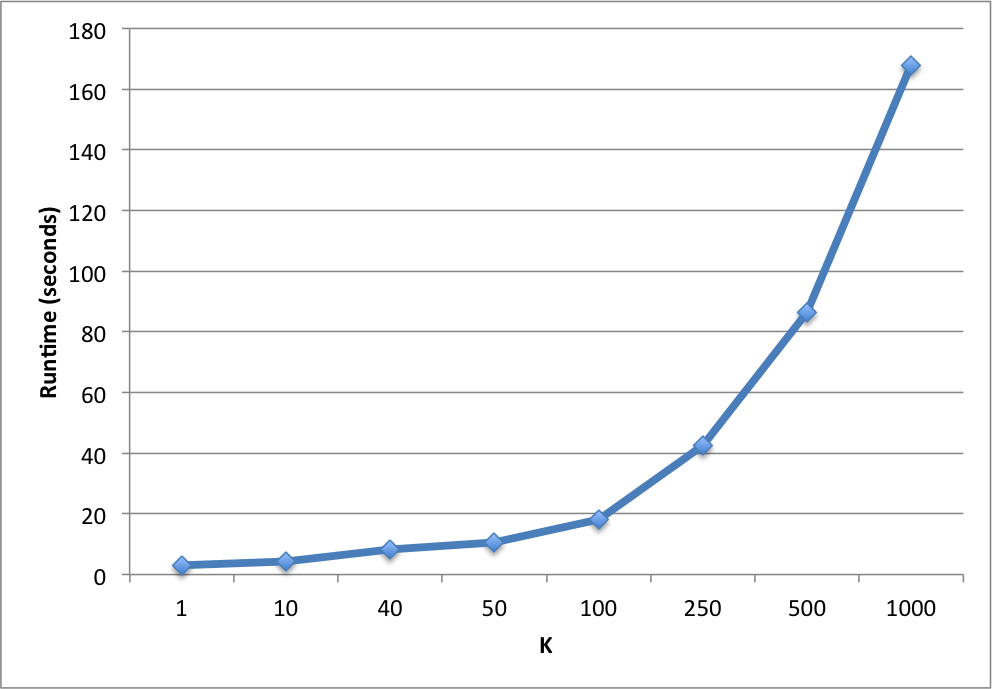
\includegraphics[width=12cm]{k-runtime}
	\caption{Runtime increases linearly with respect to K.}
	\label{fig:kruntime}
\end{figure}

Figure \ref{fig:kruntime} shows that the runtime increases linearly with respect to K. This is expected as the value of K increases, the beam search space also increases linearly.

\begin{figure}[h*]
	\centering
	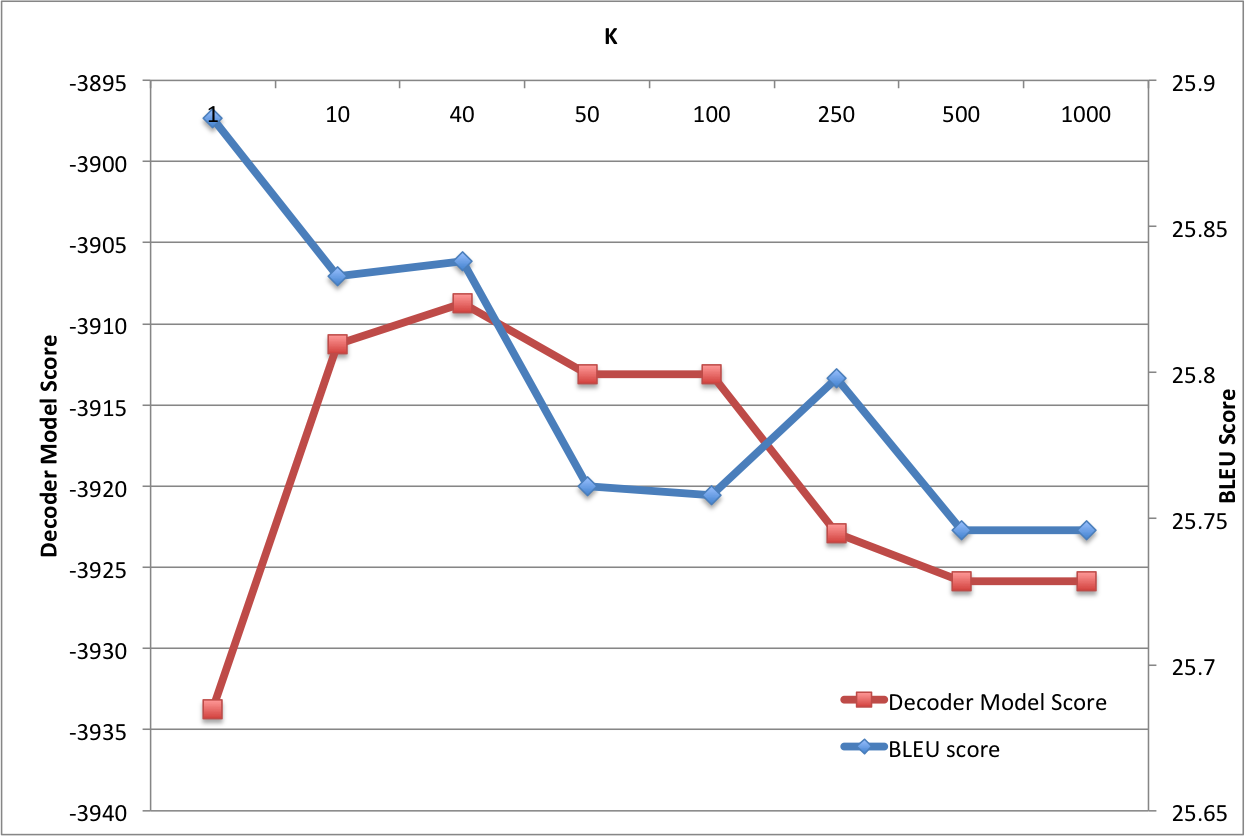
\includegraphics[width=12cm]{k-score}
	\caption{K has little effect on decoder model score and BLEU score.}
	\label{fig:kscore}
\end{figure}

Figure \ref{fig:kscore} shows that increasing temporal search space (i.e. the value of K) has little effect on the BLEU score and the model score. The data are too noisy to conclude anything but there is a weak trend of diminishing return for higher K values. This is consistent with what we learned in class. It shows more complicated algorithms do not necessarily perform better than simple, fast algorithms given large amount of data \cite{dataeffect}.

%%%%%%%%%%%%%%%%%%%%%%%%%%%%%%%%%%%%%%%%%%%%%%%%%%%%%%%%%%%%%%%%%%%%%%%%%%%%%%
%%%%%%%%%%%%%%%%%%%%%%%%%%%%%%%%%%%%%%%%%%%%%%%%%%%%%%%%%%%%%%%%%%%%%%%%%%%%%%

\section{Conclusion}
We implemented five different French-English language translation decoders using a variant of the beam search algorithm. We showed that the simple language-aware monotonic decoder gives the highest translation quality based on its BLEU score, while the distortion models are better judging by the decoder model score, although the different distortion cost functions yield little differences in the final scores. We also investigated the effect of beam search size K on BLEU scores and decoder model scores and found little correlation between the two.


%%%%%%%%%%%%%%%%%%%%%%%%%%%%%%%%%%%%%%%%%%%%%%%%%%%%%%%%%%%%%%%%%%%%%%%%%%%%%%
%%%%%%%%%%%%%%%%%%%%%%%%%%%%%%%%%%%%%%%%%%%%%%%%%%%%%%%%%%%%%%%%%%%%%%%%%%%%%%
\bibliographystyle{abbrv}
\bibliography{a2}



\end{document}












